Welcome to the
\href{https://github.com/ENSYSTRA/short-term-forecasting}{short-term-forecasting}
wiki!

Short-term forecasting of electricity generation, demand and prices
using machine learning.

Copyright (C) 2019 \href{https://nmstreethran.github.io/}{Nithiya
Streethran}.

Permission is granted to copy, distribute and/or modify this document
under the terms of the \href{https://www.gnu.org/licenses/fdl-1.3}{GNU
Free Documentation License}, Version 1.3 or any later version published
by the Free Software Foundation; with no Invariant Sections, no
Front-Cover Texts, and no Back-Cover Texts. A copy of the license is
included in the section entitled ``GNU Free Documentation License''.

Images are licensed under the
\href{https://creativecommons.org/licenses/by-sa/4.0/}{Creative Commons
Attribution-ShareAlike 4.0 International (CC BY-SA 4.0)} license, where
the image source has not been specified.

This work is part of Nithiya Streethran's research as Early-Stage
Researcher (ESR) 9 of the \href{https://ensystra.eu/}{ENSYSTRA - ENergy
SYStems in TRAnsition} Innovative Training Network. ENSYSTRA is funded
by the European Union's Horizon 2020 research and innovation programme
under the Marie Skłodowska-Curie grant agreement No: 765515.

\href{https://ensystra.eu/}{
\includegraphics[width=\textwidth,height=0.52083in]{logos/ensystra-ls.png}}~~~
\includegraphics[width=\textwidth,height=0.52083in]{logos/eu.jpg}

\hypertarget{background}{%
\section{Background}\label{background}}

The transition towards a future low-carbon economy is driven globally by
the Paris Agreement {[}Pari15{]}, which recognises the need for
sustainable development worldwide to counter the threats of climate
change. The European Union (EU) is committed to reduce greenhouse gas
(GHG) emissions by 2050 to 80-90 \% below 1990 levels {[}Ener12{]}. As
the energy industry is responsible for the highest share of
anthropogenic GHG emissions, importance is placed on how changes in
energy systems can help achieve these GHG emission reduction targets
{[}Ener12{]}.

A number of opportunities exist for the decarbonisation of the energy
industry. The International Renewable Energy Agency (IRENA), in their
renewable energy roadmap study, has identified renewable energy as
having the highest potential in reducing energy-related carbon dioxide
(CO\textsubscript{2}) emissions globally, which is closely followed by
energy efficiency and electrification with renewable energy
{[}Glob18{]}. In a 2018 political agreement, the EU member states agreed
upon a target of at least 32 \% of the demand being met with renewables
by 2030, through national targets of the individual member states
{[}ReneND{]}. The electricity demand in the transport sector is also
expected to increase due to expected petrol and diesel engine bans and
subsequently the electrification of road transport {[}Worl17{]}.

The energy system is also transitioning towards a decentralised system
with more consumer participation and new forms of flexibilities,
including sector coupling, demand-side management (DSM), energy
conversion and storage, cross-border interconnection and curtailment.
This allows demand patterns to shift to better suit the generation
patterns in systems with high penetration of variable renewable energy
(VRE) resources, such as solar and wind {[}Lund17{]}, {[}Towa18{]}.
However, this requires cooperation involving many actors with various
responsibilities and dependencies that interact within this energy
system, and opens up the opportunity to perform interdisciplinary
research work in the area of energy system analysis.

The ENSYSTRA - ENergy SYStems in TRAnsition Innovative Training Network
has been established to address the challenges of the energy transition
with interdisciplinary collaboration and regional cooperation involving
academia, government and industry {[}AbouND{]}. ENSYSTRA is centred on
the North Sea region and focusses on performing interdisciplinary
modelling work involving technology, economics, social science and
humanities, and combining various modelling approaches in different
levels and resolutions. ENSYSTRA aims to keep an open science approach,
which will allow the resulting models to be subject to full scientific
scrutiny.

Energy systems models, which are tools used to project the future energy
supply of a country or region {[}Herb12{]}, is the centre of ENSYSTRA.
The figure below explains the energy systems modelling process using a
system analysis approach {[}Kroo15{]}. This process starts with creating
a model of the actual energy system by simplifying and conceptualising
the present system. This conceptualised system with all assumptions is
then mathematically solved to produce numerical results. These results
can then be interpreted and conclusions can be drawn regarding the
future energy system. Such conclusions form the evidence-base for
decision makers, resulting in policy implications or operational
strategies that help achieve these climate targets.

\begin{figure}
\centering
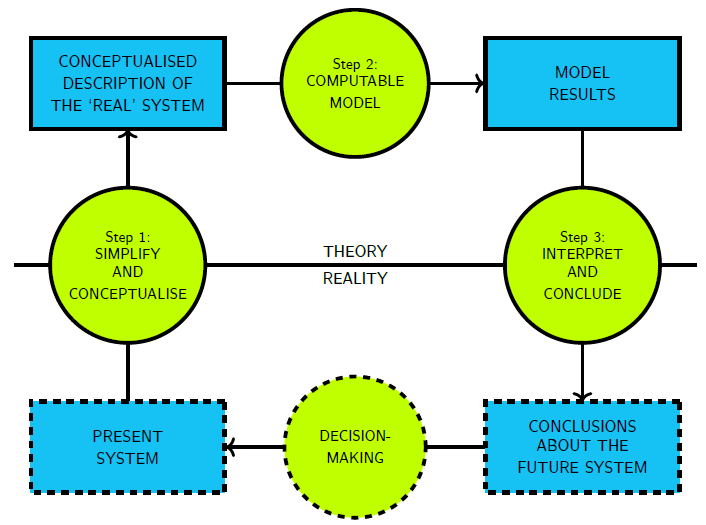
\includegraphics{images/system-analysis.png}
\caption{The system analysis approach applied on the energy system
modelling process, adapted from Krook-Riekkola 2015 {[}Kroo15{]}.}
\end{figure}

There are 15 early-stage researchers (ESRs) across four work packages
(WPs) in ENSYSTRA, as shown in the figure below. The research project
entitled ``Development of a real-time optimisation solution for
dispatchable energy supply units'' is conducted by ESR 9, who is
enrolled as a PhD student at University of Stavanger (UiS) in Norway.
This project is within WP 2 (technology prospects and development
pathways), which focusses on technological options for the energy
transition, mainly in terms of techno-economic performance over time.
For this research project, the technology focus is on the digitalisation
of the electricity sector. As the electricity system transitions into
smart systems, the system will have an increasing amount of sensors and
controllers that continuously record measurements of the system
{[}Lund17{]}. Advancements in these technologies mean that data that is
fast, heterogeneous and high in volume from the electricity system will
be generated. Data with these characteristics must be managed and
analysed effectively to gain insights on the electricity system, which
can then be converted to strategies that optimise the system
{[}Mana12{]}. This project will specifically investigate how artificial
intelligence (AI) can play a role in the transition to a low-carbon
electricity system by utilising high resolution data of the system. The
next section will investigate this, as well as explain what is meant by
``real-time'' and ``dispatchable'' in the context of electricity systems
in this project.

\begin{figure}
\centering
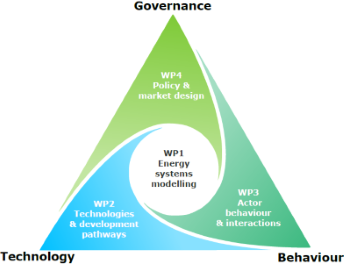
\includegraphics{images/wp.png}
\caption{Interactions between the four WPs of the ENSYSTRA project.
Source: ENSYSTRA {[}AbouND{]}.}
\end{figure}

\hypertarget{problem-definition}{%
\section{Problem definition}\label{problem-definition}}

\hypertarget{electricity-system}{%
\subsection{Electricity system}\label{electricity-system}}

The electricity system can be seen as having two components; the
physical grid consisting of generators and transmission and distribution
systems, and the electricity market consisting of a number of actors
{[}Erba16{]}.

Electricity systems exist in different resolutions and levels of
uncertainty. The figure below represents the different scales of
electricity systems, mainly in terms of temporal resolution, but also
uncertainty and spatial resolution {[}Glis18{]}, {[}Pfen14{]}.
Temporally, ``real-time'' is referred to as the time of dispatch. It can
be observed that the operational planning scale has high spatial and
temporal resolution, and relatively low uncertainty. Operational
planning includes dispatch planning and plant scheduling (i.e., unit
commitment), which ranges from a few minutes to a week before dispatch.
Maintenance planning can take a few weeks to years, as it involves
upgrade and maintenance work which may require shut-down of units or
assets, in turn affecting the availability of generation units and grid
infrastructure. Adequacy assessments, which takes years, involve
assessing the existing generation and storage capacities and planning
for new installations based on demand projections, to ensure this demand
will be met in the future. Finally, grid investment decisions, including
planning transmission and distribution grid networks, cross-border and
regional interconnections and grid capacity expansions, take many years
to decades and have very high uncertainty as a result.

\begin{figure}
\centering
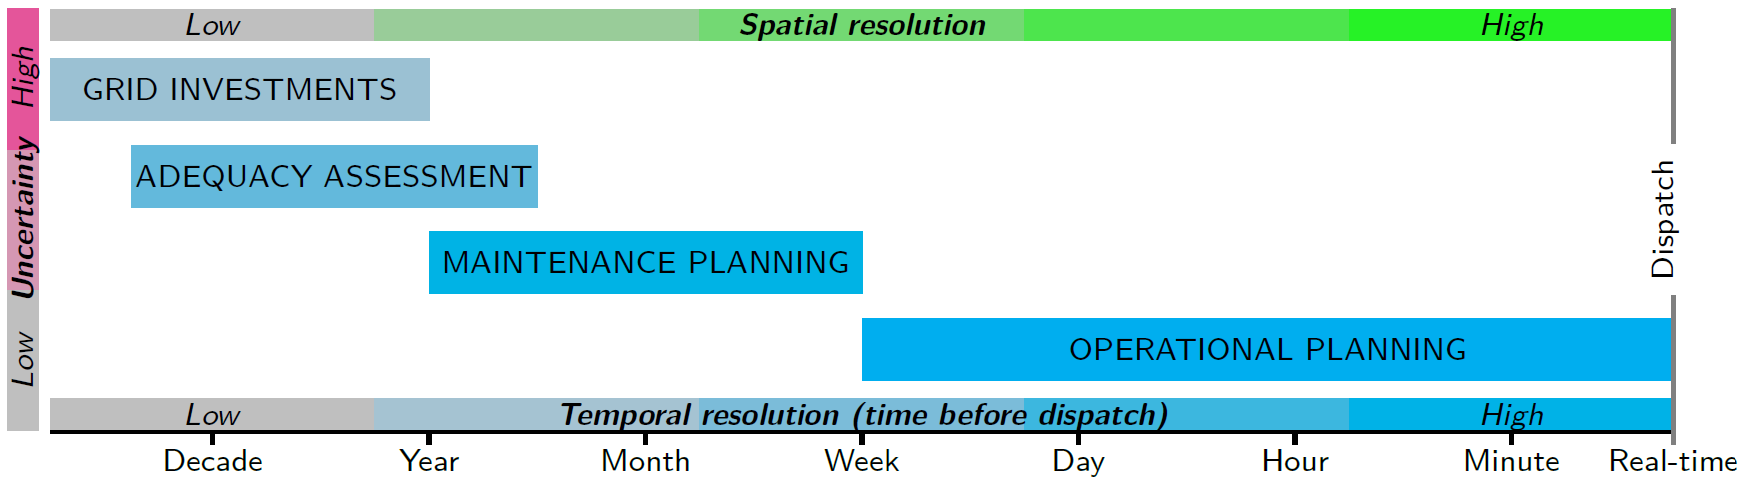
\includegraphics{images/resolution.png}
\caption{The various scales of electricity systems in terms of their
approximate temporal resolution, as well as spatial resolution and
uncertainty, adapted from Glismann 2018 and Pfenninger, et al.~2014
{[}Glis18{]}, {[}Pfen14{]}.}
\end{figure}

\hypertarget{generation-technologies}{%
\subsection{Generation technologies}\label{generation-technologies}}

The table below shows the characteristics of the main energy generation
technologies, including their costs. These generation sources have
different variabilities, fuel types, flexibilities, costs and carbon
emissions. According to the EU reference scenario 2016 {[}EnerND{]},
wind and solar energy resources, which are VRE resources, are expected
to generate a total of 35 \% of EU's electricity by 2050, which is a
significant increase (23 \%) from 2015 levels. Conversely, generation
from nuclear and solids, which are not variable and provide base load
generation, are expected to decrease significantly. Unlike conventional
generators, VRE are intermittent as they are dependent on atmospheric
conditions, such as wind speed and cloud cover, and they vary both
spatially (i.e., location-dependent) and temporally {[}Josk11{]}.
Therefore, VRE generation cannot be controlled to meet the demand
patterns and needs of the energy system {[}Josk11{]}, which is a
challenge to electricity and energy system operators in general. The
costs listed in this table are derived based on National Renewable
Energy Laboratory (NREL)'s NREL-SEAC 2008 Data Set {[}Tidb10{]}. VRE
generation technologies have high capital expenditure (CAPEX) compared
to conventional fossil-powered and biomass generation. Conversely, the
operational expenditure (OPEX), which includes fuel and fixed
operational and maintenance (O\&M) costs, is low for VRE generation
technologies, as they have no fuel costs unlike conventional generators.

\begin{longtable}[]{@{}llllllll@{}}
\caption{Characteristics of the main energy generation technologies,
adapted from Erbach 2016 {[}Erba16{]} and Tidball, et al.~2010
{[}Tidb10{]}.}\tabularnewline
\toprule
Type\textsuperscript{\protect\hyperlink{f1}{{[}f1{]}}} & Variable & Fuel
type & Flexibility & Low carbon & CAPEX & OPEX &
LCOE\textsuperscript{\protect\hyperlink{f2}{{[}f2{]}}}\tabularnewline
\midrule
\endfirsthead
\toprule
Type\textsuperscript{\protect\hyperlink{f1}{{[}f1{]}}} & Variable & Fuel
type & Flexibility & Low carbon & CAPEX & OPEX &
LCOE\textsuperscript{\protect\hyperlink{f2}{{[}f2{]}}}\tabularnewline
\midrule
\endhead
Coal & no & fossil & medium & no & low & high & very low\tabularnewline
Natural gas & no & fossil & high & no & very low & very high &
low\tabularnewline
Biomass & no & renewable & medium &
yes\textsuperscript{\protect\hyperlink{f3}{{[}f3{]}}} & low & very high
& very high\tabularnewline
Nuclear & no & nuclear & low & zero-emission & medium & medium &
medium\tabularnewline
Hydro & no & renewable & very high & zero-emission & & &\tabularnewline
Solar & yes & renewable & very low & zero-emission & very high & very
low & very high\tabularnewline
Wind & yes & renewable & very low & zero-emission & & &\tabularnewline
\emph{Onshore wind} & & & & & high & very low & very low\tabularnewline
\emph{Offshore wind} & & & & & very high & low & high\tabularnewline
Geothermal & no & renewable & high & zero-emission & high & medium &
high\tabularnewline
\bottomrule
\end{longtable}

\protect\hypertarget{f1}{}{{[}f1{]}} \emph{Costs for natural gas,
biomass, solar and geothermal are that of advanced combustion turbine,
biomass gasification plant, utility-scale photovoltaic and hydrothermal
plant respectively}

\protect\hypertarget{f2}{}{{[}f2{]}} \emph{LCOE - levelised cost of
electricity}

\protect\hypertarget{f3}{}{{[}f3{]}} \emph{regrowth of biomass
compensates emissions}

\hypertarget{electricity-market}{%
\subsection{Electricity market}\label{electricity-market}}

The actors in the electricity market include {[}Erba16{]}, {[}PinsND{]},
{[}TheC15{]}:

\begin{itemize}
\tightlist
\item
  Generator
\item
  Retailer
\item
  Large and small consumer
\item
  Transmission system operator (TSO)
\item
  Distribution network operator (DNO)
\item
  Balance responsible party (BRP)
\item
  Aggregator
\item
  Regulator
\item
  Market operator
\end{itemize}

There are two types of electricity markets; the retail market and the
wholesale market {[}Erba16{]}. The retail market involves the retailers
buying electricity from generators and selling it to consumers. The
wholesale market involves generators, retailers and (large) consumers,
who buy and sell electricity. Energy-only transactions in the wholesale
market have different temporal resolutions {[}PinsND{]}, {[}TheC15{]}
and take place before dispatch, shown in green in the figure below.
Balancing markets, shown in pink in the figure below, which involve both
energy and services, operate both before and after dispatch
{[}TheC15{]}. The energy-only markets are operated by the market
operator or power exchanges, while the balancing market is operated by
the system operator. The day-ahead and intra-day markets can be
considered short-term electricity markets, as the former takes place 24
hours in advance of dispatch, while the latter takes place continuously
after the day-ahead market, up to minutes before dispatch {[}Over16{]}.

\begin{figure}
\centering
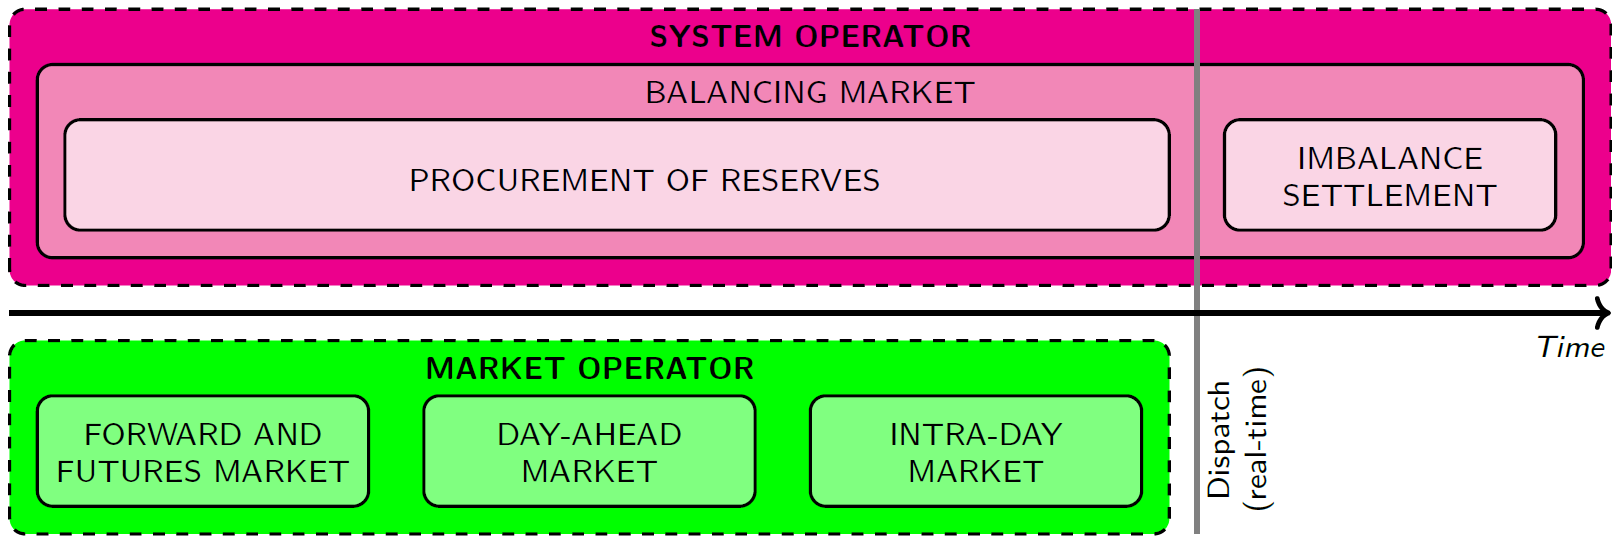
\includegraphics{images/market-resolution.png}
\caption{The various electricity markets in terms of operator and
temporal resolution, before and after dispatch, adapted from KU Leuven
Energy Institute 2015 and Pinson 2018 {[}PinsND{]}, {[}TheC15{]}.}
\end{figure}

\hypertarget{objectives}{%
\section{Objectives}\label{objectives}}

The main research objective of this project is:

\begin{quote}
\emph{To develop an open-source, machine learning-based electricity
market model for the North Sea region which will help electricity
generators, retailers, large consumers, BRPs and system operators in
short-term electricity markets (i.e., day-ahead and intra-day markets)
to develop operational and bidding strategies that maximise their
profits under uncertainty of VRE generation. The model will consist of a
forecaster based on machine learning, which will use high resolution
time series weather forecasts for the upcoming period, and recent
historical measurements of electricity generation, demand and market
prices, to forecast the latter three quantities for the upcoming period.
These forecasts will serve as inputs to an optimiser, which maximises
social welfare in the electricity market.}
\end{quote}

Based on the main research objective, the following research questions
have been derived:

\begin{itemize}
\tightlist
\item
  What methods and resources are needed to process and store the large
  volume of high resolution data required for this model?
\item
  What type of machine learning algorithms are suited for the time
  series forecasting of electricity prices, demand and generation?
\item
  What optimisation methods are suitable for maximising the social
  welfare problem in the electricity market, and what are the
  constraints to this optimisation problem?
\item
  What methods can be used to analyse the inputs and outputs of the
  model and translate them into operational strategies relevant to the
  market participant?
\item
  How can this model be standardised and published so that it is
  available for use openly by any participant in the electricity market,
  as well as other interested parties, such as policymakers?
\item
  How can this high resolution electricity market operational model be
  integrated with the overall North Sea energy systems model to provide
  insights on long-term planning and investments in the energy sector?
\end{itemize}

\hypertarget{regions}{%
\section{Regions}\label{regions}}

\hypertarget{north-sea-countries}{%
\subsection{North Sea countries}\label{north-sea-countries}}

As per the definition provided by the European MSP Platform {[}NortND{]}
and the CPMR North Sea Commission {[}Memb15{]}, the North Sea region
consists of eight countries: Belgium, Denmark, France, Germany,
Netherlands, Norway, Sweden and United Kingdom.

\hypertarget{nuts-nomenclature-of-territorial-units-for-statistics}{%
\subsubsection{\texorpdfstring{\href{https://ec.europa.eu/eurostat/web/nuts/background}{NUTS
(Nomenclature of territorial units for
statistics)}}{NUTS (Nomenclature of territorial units for statistics)}}\label{nuts-nomenclature-of-territorial-units-for-statistics}}

\href{https://github.com/ENSYSTRA/short-term-forecasting/tree/master/jupyter-notebooks/NUTS.ipynb}{See
the Jupyter notebook}.

\hypertarget{bidding-zones}{%
\subsection{Bidding zones}\label{bidding-zones}}

\hypertarget{definition}{%
\subsubsection{Definition}\label{definition}}

According to {[}Bidd14{]}:

\begin{itemize}
\tightlist
\item
  The largest geographical area within which market participants are
  able to exchange energy without capacity allocation.
\item
  The majority of bidding zones in Europe are defined by national
  borders (e.g., France or the Netherlands).
\item
  Some are larger than national borders (e.g., Austria, Germany and
  Luxembourg or the Single Electricity Market for the island of Ireland)
\item
  Some are smaller zones within individual countries (e.g., Italy,
  Norway or Sweden).
\end{itemize}

\hypertarget{bidding-zones-in-the-north-sea-region}{%
\subsubsection{Bidding zones in the North Sea
region}\label{bidding-zones-in-the-north-sea-region}}

The bidding zones in the European electricity market are illustrated in
the map below {[}Tren17{]}.

\begin{figure}
\centering
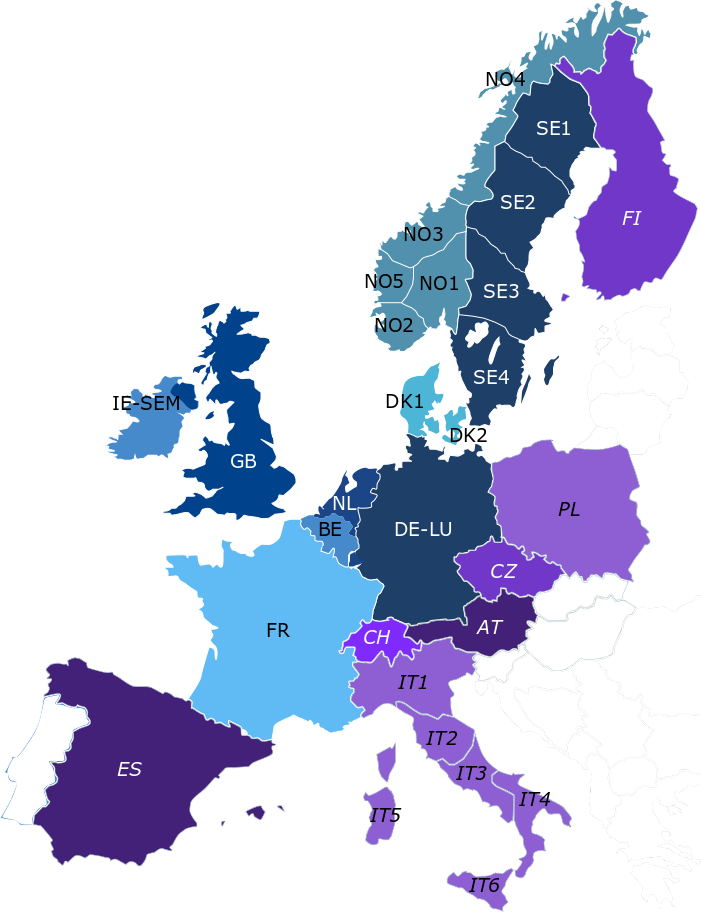
\includegraphics{images/market-map.png}
\caption{Bidding zones in the European electricity market. Source:
\href{http://raport.pse.pl/en/trends-and-market-context}{Polskie Sieci
Elektroenergetyczne} {[}Tren17{]}.}
\end{figure}

\begin{longtable}[]{@{}lll@{}}
\caption{Bidding zones in the North Sea region.}\tabularnewline
\toprule
\textbf{Country} & \textbf{Market(s)} & \textbf{Zone(s)}\tabularnewline
\midrule
\endfirsthead
\toprule
\textbf{Country} & \textbf{Market(s)} & \textbf{Zone(s)}\tabularnewline
\midrule
\endhead
Belgium (BE) & EPEX SPOT & BE\tabularnewline
Germany (DE / GE) & EPEX SPOT &
DE-AT-LU\textsuperscript{\protect\hyperlink{f4}{{[}f4{]}}}\tabularnewline
Denmark (DK) & Nord Pool & DK1, DK2\tabularnewline
France (FR) & EPEX SPOT & FR\tabularnewline
Netherlands (NL) & EPEX SPOT & NL\tabularnewline
Norway (NO) & Nord Pool & NO1, NO2, NO3, NO4, NO5\tabularnewline
Sweden (SE / SW) & Nord Pool & SE1, SE2, SE3, SE4\tabularnewline
United Kingdom (UK) & EPEX SPOT, Nord Pool & GB,
I-SEM\textsuperscript{\protect\hyperlink{f4}{{[}f4{]}}}\tabularnewline
\bottomrule
\end{longtable}

\protect\hypertarget{f4}{}{{[}f4{]}} \emph{Austria (AT / AU); Luxembourg
(LU); Great Britain (GB); Irish single electricity market (I-SEM), which
includes Republic of Ireland (IE) and UK's Northern Ireland (NI).}

\hypertarget{transmission-system-operators-and-interconnections}{%
\subsubsection{Transmission system operators and
interconnections}\label{transmission-system-operators-and-interconnections}}

The power exchanges that operate in the North Sea region are EPEX SPOT
(Belgium, France, Germany, Netherlands, United Kingdom) and Nord Pool
(Denmark, Norway, Sweden, United Kingdom) {[}Over16{]}, {[}SeeMND{]},
{[}EPEXND{]}. The day-ahead market takes place generally as an hourly
auction 24 hours prior to dispatch {[}Over16{]}. The intra-day market
has continuous trading and will operate until two hours and up to five
minutes before dispatch {[}Over16{]}. The North Sea region consists of
multiple TSOs, cross-border interconnections and bidding zones, as
listed in the table below.

\begin{longtable}[]{@{}llll@{}}
\caption{TSOs and cross-border interconnections in the North Sea region.
Data: European Network of Transmission System Operators for Electricity
{[}ENTSND{]}, {[}RegiND{]}.}\tabularnewline
\toprule
\begin{minipage}[b]{0.07\columnwidth}\raggedright
Ctry.\textsuperscript{\protect\hyperlink{f5}{{[}f5{]}}}\strut
\end{minipage} & \begin{minipage}[b]{0.36\columnwidth}\raggedright
TSOs\strut
\end{minipage} & \begin{minipage}[b]{0.22\columnwidth}\raggedright
Cross-border
interconnection\textsuperscript{\protect\hyperlink{f5}{{[}f5{]}},\protect\hyperlink{f6}{{[}f6{]}}}\strut
\end{minipage} & \begin{minipage}[b]{0.22\columnwidth}\raggedright
Bidding
zones\textsuperscript{\protect\hyperlink{f5}{{[}f5{]}},\protect\hyperlink{f6}{{[}f6{]}}}\strut
\end{minipage}\tabularnewline
\midrule
\endfirsthead
\toprule
\begin{minipage}[b]{0.07\columnwidth}\raggedright
Ctry.\textsuperscript{\protect\hyperlink{f5}{{[}f5{]}}}\strut
\end{minipage} & \begin{minipage}[b]{0.36\columnwidth}\raggedright
TSOs\strut
\end{minipage} & \begin{minipage}[b]{0.22\columnwidth}\raggedright
Cross-border
interconnection\textsuperscript{\protect\hyperlink{f5}{{[}f5{]}},\protect\hyperlink{f6}{{[}f6{]}}}\strut
\end{minipage} & \begin{minipage}[b]{0.22\columnwidth}\raggedright
Bidding
zones\textsuperscript{\protect\hyperlink{f5}{{[}f5{]}},\protect\hyperlink{f6}{{[}f6{]}}}\strut
\end{minipage}\tabularnewline
\midrule
\endhead
\begin{minipage}[t]{0.07\columnwidth}\raggedright
BE\strut
\end{minipage} & \begin{minipage}[t]{0.36\columnwidth}\raggedright
Elia System Operator\strut
\end{minipage} & \begin{minipage}[t]{0.22\columnwidth}\raggedright
FR, LU, NL, UK\strut
\end{minipage} & \begin{minipage}[t]{0.22\columnwidth}\raggedright
BE\strut
\end{minipage}\tabularnewline
\begin{minipage}[t]{0.07\columnwidth}\raggedright
DK\strut
\end{minipage} & \begin{minipage}[t]{0.36\columnwidth}\raggedright
Energinet\strut
\end{minipage} & \begin{minipage}[t]{0.22\columnwidth}\raggedright
DE, NO, SE\strut
\end{minipage} & \begin{minipage}[t]{0.22\columnwidth}\raggedright
DK1, DK2\strut
\end{minipage}\tabularnewline
\begin{minipage}[t]{0.07\columnwidth}\raggedright
DE\strut
\end{minipage} & \begin{minipage}[t]{0.36\columnwidth}\raggedright
TransnetBW, TenneT TSO, Amprion, 50Hertz Transmission\strut
\end{minipage} & \begin{minipage}[t]{0.22\columnwidth}\raggedright
AT, CH, CZ, DK, FR, LU, NL, PL, SE\strut
\end{minipage} & \begin{minipage}[t]{0.22\columnwidth}\raggedright
CZ+DE+SK, DE-AT-LU, DE-LU\strut
\end{minipage}\tabularnewline
\begin{minipage}[t]{0.07\columnwidth}\raggedright
FR\strut
\end{minipage} & \begin{minipage}[t]{0.36\columnwidth}\raggedright
Réseau de Transport d'Electricité\strut
\end{minipage} & \begin{minipage}[t]{0.22\columnwidth}\raggedright
BE, CH, DE, ES, IT, UK\strut
\end{minipage} & \begin{minipage}[t]{0.22\columnwidth}\raggedright
FR\strut
\end{minipage}\tabularnewline
\begin{minipage}[t]{0.07\columnwidth}\raggedright
NL\strut
\end{minipage} & \begin{minipage}[t]{0.36\columnwidth}\raggedright
TenneT TSO\strut
\end{minipage} & \begin{minipage}[t]{0.22\columnwidth}\raggedright
BE, DE, NO, UK\strut
\end{minipage} & \begin{minipage}[t]{0.22\columnwidth}\raggedright
NL\strut
\end{minipage}\tabularnewline
\begin{minipage}[t]{0.07\columnwidth}\raggedright
NO\strut
\end{minipage} & \begin{minipage}[t]{0.36\columnwidth}\raggedright
Statnett\strut
\end{minipage} & \begin{minipage}[t]{0.22\columnwidth}\raggedright
DK, FI, NL, SE\strut
\end{minipage} & \begin{minipage}[t]{0.22\columnwidth}\raggedright
NO1, NO2, NO3, NO4, NO5\strut
\end{minipage}\tabularnewline
\begin{minipage}[t]{0.07\columnwidth}\raggedright
SE\strut
\end{minipage} & \begin{minipage}[t]{0.36\columnwidth}\raggedright
Svenska Kraftnät\strut
\end{minipage} & \begin{minipage}[t]{0.22\columnwidth}\raggedright
DK, FI, DE, LT, NO, PL\strut
\end{minipage} & \begin{minipage}[t]{0.22\columnwidth}\raggedright
SE1, SE2, SE3, SE4\strut
\end{minipage}\tabularnewline
\begin{minipage}[t]{0.07\columnwidth}\raggedright
UK\strut
\end{minipage} & \begin{minipage}[t]{0.36\columnwidth}\raggedright
National Grid Electricity Transmission, System Operator for Northern
Ireland, Scottish Hydro Electric Transmission, ScottishPower
Transmission\strut
\end{minipage} & \begin{minipage}[t]{0.22\columnwidth}\raggedright
BE, FR, IE, NL\strut
\end{minipage} & \begin{minipage}[t]{0.22\columnwidth}\raggedright
GB, IE (SEM)\strut
\end{minipage}\tabularnewline
\bottomrule
\end{longtable}

\protect\hypertarget{f5}{}{{[}f5{]}} \emph{Ctry. - Country; AT -
Austria; BE - Belgium; CH - Switzerland; CZ - Czech Republic; DE -
Germany; DK - Denmark; ES - Spain; FI - Finland; FR - France; GB - Great
Britain; IE - Ireland; IT - Italy; LT - Lithuania; LU - Luxembourg; NL -
Netherlands; NO - Norway; PL - Poland; SE - Sweden; SK - Slovakia; UK -
United Kingdom; SEM - Single electricity market.}

\protect\hypertarget{f6}{}{{[}f6{]}} \emph{These countries are not part
of the North Sea region: AT, CH, CZ, ES, FI, IE, IT, LT, LU, PL.}

\hypertarget{data}{%
\section{Data}\label{data}}

\hypertarget{data-folder-navigation}{%
\subsection{\texorpdfstring{\href{https://drive.google.com/drive/folders/1_3Y30j_c-4iai0WuhcrysXHYdZ4F2AKB}{Data
folder}
navigation}{Data folder navigation}}\label{data-folder-navigation}}

\begin{itemize}
\tightlist
\item
  ENTSO-E

  \begin{itemize}
  \tightlist
  \item
    generation and load data for each bidding zone in the North Sea
    region, grouped by country
  \end{itemize}
\item
  Meteo - meteorological data, grouped by country
\item
  Market - market data for the North Sea region
\item
  NUTS - territorial units
\item
  output - output or modified data from this project
\end{itemize}

\hypertarget{met-data}{%
\subsection{Met data}\label{met-data}}

\hypertarget{deutscher-wetterdienst}{%
\paragraph{\texorpdfstring{\href{https://www.dwd.de/EN/climate_environment/cdc/cdc_node.html}{Deutscher
Wetterdienst}}{Deutscher Wetterdienst}}\label{deutscher-wetterdienst}}

\begin{itemize}
\tightlist
\item
  \href{https://cdc.dwd.de/portal/}{CDC (Climate Data Center) portal}
\item
  \href{https://opendata.dwd.de/climate_environment/CDC/}{CDC OpenData}
\item
  \href{https://opendata.dwd.de/climate_environment/CDC/Terms_of_use.pdf}{Terms
  of use for data on the CDC ftp server}
\item
  Data set descriptions

  \begin{itemize}
  \tightlist
  \item
    \href{https://cdc.dwd.de/sdi/pid/TT_TU_MN009/DESCRIPTION_TT_TU_MN009_en.pdf}{Hourly
    station observations of air temperature at 2 m above ground in °C
    for Germany}
  \item
    \href{https://cdc.dwd.de/sdi/pid/RF_TU_MN009/DESCRIPTION_RF_TU_MN009_en.pdf}{Hourly
    station observations of relative humidity in \% for Germany}
  \item
    \href{https://cdc.dwd.de/sdi/pid/R1_MN008/DESCRIPTION_R1_MN008_en.pdf}{Hourly
    station observations of precipitation amount in mm for Germany}
  \item
    \href{https://cdc.dwd.de/sdi/pid/WRTR_MN008/DESCRIPTION_WRTR_MN008_en.pdf}{Hourly
    station observations of form of precipitation (WR code) for Germany}
  \item
    \href{https://cdc.dwd.de/sdi/pid/RS_IND_MN008/DESCRIPTION_RS_IND_MN008_en.pdf}{Hourly
    station observations of index whether precipitation has fallen for
    Germany}
  \item
    \href{https://cdc.dwd.de/sdi/pid/F_MN003/DESCRIPTION_F_MN003_en.pdf}{Hourly
    mean of station observations of wind speed ca. 10 m above ground in
    m/s for Germany}
  \item
    \href{https://cdc.dwd.de/sdi/pid/D_MN003/DESCRIPTION_D_MN003_en.pdf}{Hourly
    mean of station observations of wind direction at ca. 10 m above
    ground in degree for Germany}
  \item
    \href{https://cdc.dwd.de/sdi/pid/P0_MN008/DESCRIPTION_P0_MN008_en.pdf}{Hourly
    station observations of air pressure at station level in hpa for
    Germany}
  \item
    \href{https://cdc.dwd.de/sdi/pid/P_MN008/DESCRIPTION_P_MN008_en.pdf}{Hourly
    station observations of air pressure at mean sea level in hpa for
    Germany}
  \item
    \href{https://cdc.dwd.de/sdi/pid/N_MN008/DESCRIPTION_N_MN008_en.pdf}{Hourly
    station observations of cloud coverage in eighths for Germany}
  \end{itemize}
\item
  \href{https://opendata.dwd.de/climate_environment/CDC/observations_germany/climate/hourly/wind/}{Hourly
  wind data}
\end{itemize}

\hypertarget{royal-netherlands-meteorological-institute}{%
\paragraph{\texorpdfstring{\href{https://data.knmi.nl/datasets}{Royal
Netherlands Meteorological
Institute}}{Royal Netherlands Meteorological Institute}}\label{royal-netherlands-meteorological-institute}}

\hypertarget{met-office}{%
\paragraph{\texorpdfstring{\href{https://www.metoffice.gov.uk/datapoint}{Met
Office}}{Met Office}}\label{met-office}}

\hypertarget{norwegian-meteorological-institute}{%
\paragraph{\texorpdfstring{\href{https://www.met.no/en/free-meteorological-data}{Norwegian
Meteorological
Institute}}{Norwegian Meteorological Institute}}\label{norwegian-meteorological-institute}}

\hypertarget{swedish-meteorological-and-hydrological-institute}{%
\paragraph{\texorpdfstring{\href{https://www.smhi.se/en/services/professional-services/data-and-statistics}{Swedish
Meteorological and Hydrological
Institute}}{Swedish Meteorological and Hydrological Institute}}\label{swedish-meteorological-and-hydrological-institute}}

\hypertarget{danish-meteorological-institute}{%
\paragraph{\texorpdfstring{\href{http://research.dmi.dk/data/}{Danish
Meteorological
Institute}}{Danish Meteorological Institute}}\label{danish-meteorological-institute}}

\hypertarget{muxe9tuxe9o-france}{%
\paragraph{\texorpdfstring{\href{https://donneespubliques.meteofrance.fr/}{Météo-France}}{Météo-France}}\label{muxe9tuxe9o-france}}

\hypertarget{the-royal-meteorological-institute-of-belgium}{%
\paragraph{\texorpdfstring{\href{https://opendata.meteo.be/}{The Royal
Meteorological Institute of
Belgium}}{The Royal Meteorological Institute of Belgium}}\label{the-royal-meteorological-institute-of-belgium}}

\hypertarget{generation-and-demand-data}{%
\subsection{Generation and demand
data}\label{generation-and-demand-data}}

\hypertarget{entso-e-transparency-platform}{%
\paragraph{\texorpdfstring{\href{https://transparency.entsoe.eu/}{ENTSO-E
Transparency
Platform}}{ENTSO-E Transparency Platform}}\label{entso-e-transparency-platform}}

\begin{itemize}
\tightlist
\item
  \href{https://docstore.entsoe.eu/Documents/MC\%20documents/Transparency\%20Platform/ENTSOE_Transparency_Terms_Conditions.pdf}{GENERAL
  TERMS AND CONDITIONS FOR THE USE OF THE ENTSO-E TRANSPARENCY PLATFORM}
\item
  \href{https://docstore.entsoe.eu/Documents/MC\%20documents/Transparency\%20Platform/List_of_Data_available_for_reuse.pdf}{LIST
  OF DATA AVAILABLE FOR FREE RE-USE}
\item
  Downloaded data:

  \begin{itemize}
  \tightlist
  \item
    \href{https://transparency.entsoe.eu/generation/r2/actualGenerationPerProductionType/show}{Actual
    Generation per Production Type}
  \item
    \href{https://transparency.entsoe.eu/load-domain/r2/totalLoadR2/show}{Total
    Load - Day Ahead / Actual}
  \end{itemize}
\end{itemize}

\hypertarget{market-data}{%
\subsection{Market data}\label{market-data}}

\hypertarget{nord-pool}{%
\paragraph{\texorpdfstring{\href{https://www.nordpoolgroup.com/historical-market-data/}{Nord
Pool}}{Nord Pool}}\label{nord-pool}}

\begin{itemize}
\tightlist
\item
  \href{https://www.nordpoolgroup.com/trading/join-our-markets/membership/}{Membership
  list - Nord Pool}
\item
  \href{https://www.nordpoolgroup.com/About-us/Terms-and-conditions-for-use/}{Terms
  and conditions for use}
\end{itemize}

\hypertarget{epex-spot}{%
\paragraph{\texorpdfstring{\href{https://www.epexspot.com/en/extras/download-center/market_data}{EPEX
Spot}}{EPEX Spot}}\label{epex-spot}}

\begin{itemize}
\tightlist
\item
  \href{https://www.epexspot.com/en/membership/list_of_members}{EPEX
  SPOT Exchange Members}
\end{itemize}

\hypertarget{other-data}{%
\subsection{Other data}\label{other-data}}

\hypertarget{nuts-nomenclature-of-territorial-units-for-statistics-1}{%
\paragraph{\texorpdfstring{\href{https://ec.europa.eu/eurostat/web/gisco/geodata/reference-data/administrative-units-statistical-units/nuts}{NUTS
(Nomenclature of territorial units for
statistics)}}{NUTS (Nomenclature of territorial units for statistics)}}\label{nuts-nomenclature-of-territorial-units-for-statistics-1}}

\hypertarget{methodology}{%
\section{Methodology}\label{methodology}}

\hypertarget{modelling-framework}{%
\subsection{Modelling framework}\label{modelling-framework}}

\begin{figure}
\centering
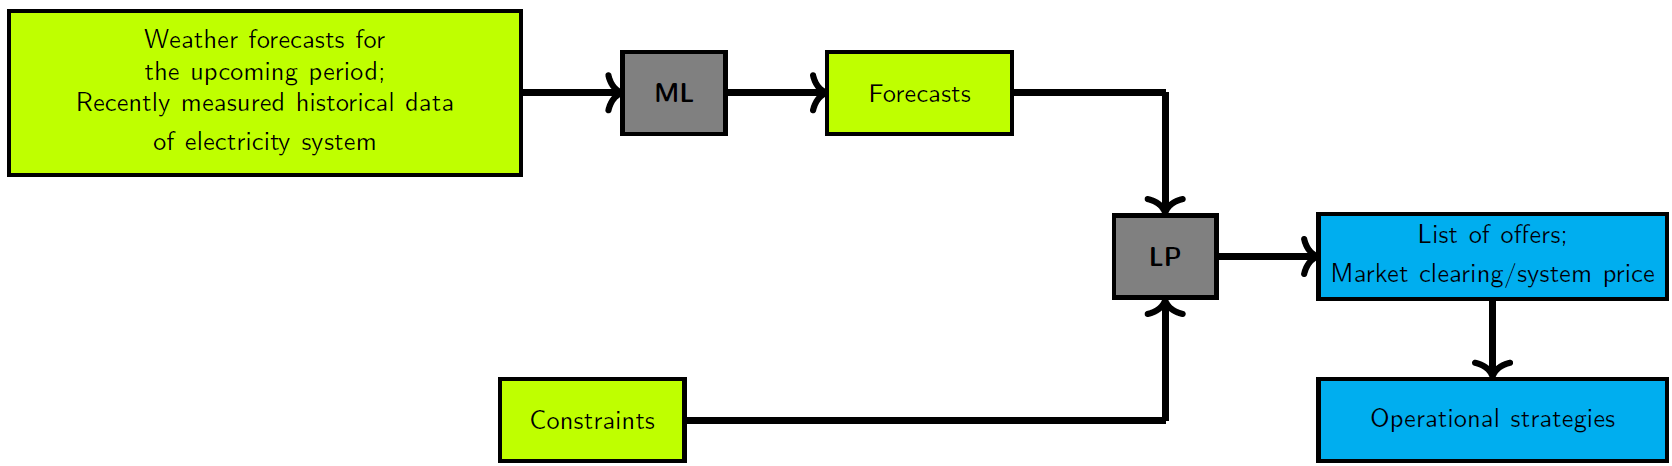
\includegraphics{images/model_framework.png}
\caption{Modelling framework. License: CC BY-SA 4.0.}
\end{figure}

\hypertarget{glossary}{%
\section{Glossary}\label{glossary}}

\hypertarget{abbreviations}{%
\subsection{Abbreviations}\label{abbreviations}}

\begin{itemize}
\tightlist
\item
  AI - artificial intelligence
\item
  BRP - balance responsible party
\item
  CAPEX - capital expenditure
\item
  CO\textsubscript{2} - carbon dioxide
\item
  COMPETES - COmprehensive Market Power in Electricity Transmission and
  Energy Simulator
\item
  DC - direct current
\item
  DNO - distribution network operator
\item
  DSM - demand-side management
\item
  EMMA - The European Electricity Market Model
\item
  ENSYSTRA - ENergy SYStems in TRAnsition
\item
  ENTSO-E - European Network of Transmission Systems Operators for
  Electricity
\item
  ESR - early-stage researcher
\item
  ETSAP - Energy Technology Systems Analysis Program
\item
  EU - European Union
\item
  GAMS - General Algebraic Modeling System
\item
  GHG - greenhouse gas
\item
  IEA - International Energy Agency
\item
  IRENA - International Renewable Energy Agency
\item
  IRiE - Integrated Regulating power market in Europe
\item
  JRC-IDEES - Joint Research Centre Integrated Database of the European
  Energy System
\item
  MARKAL - MARKet ALlocation
\item
  NREL - National Renewable Energy Laboratory
\item
  O\&M - operation and maintenance
\item
  openmod - Open Energy Modelling Initiative
\item
  OPEX - operational expenditure
\item
  PCR - Price Coupling of Regions
\item
  PhD - Doctor of Philosophy
\item
  renpass - Renewable Energy Pathways Simulation System
\item
  stELMOD - Stochastic Electricity Market Model
\item
  TIMES - The Integrated MARKAL-EFOM System
\item
  TSO - transmission system operator
\item
  UiS - University of Stavanger
\item
  VRE - variable renewable energy
\item
  WP - work package
\end{itemize}
